% Created by tikzDevice version 0.12.6 on 2024-06-11 19:56:47
% !TEX encoding = UTF-8 Unicode
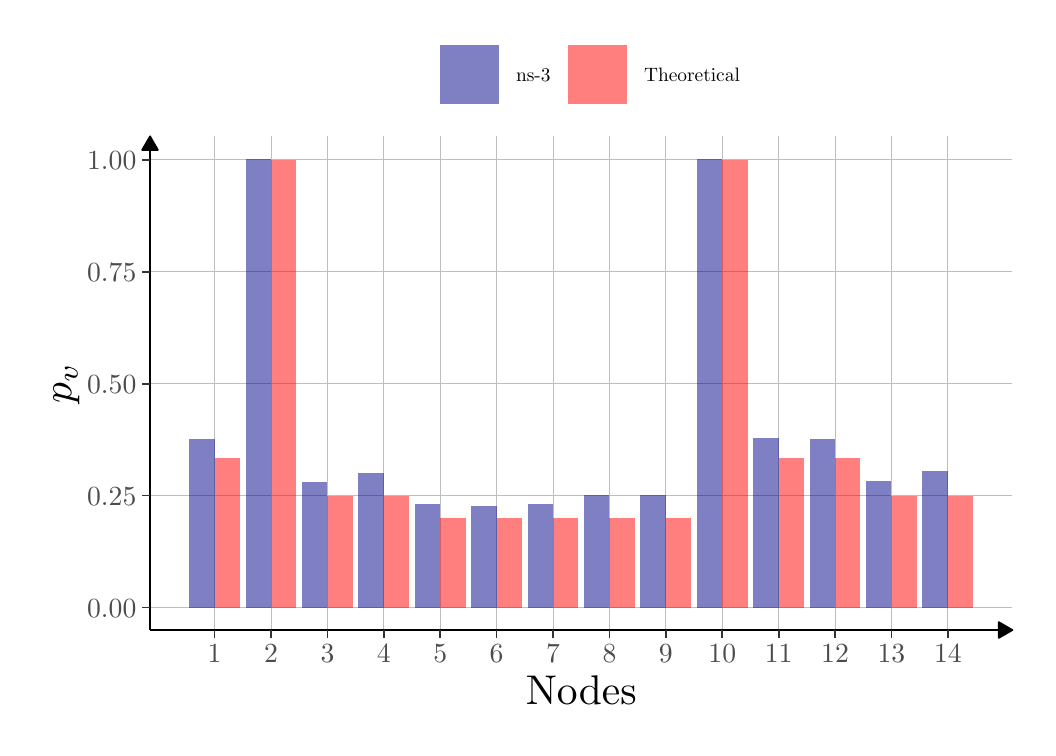
\begin{tikzpicture}[x=1pt,y=1pt]
\definecolor{fillColor}{RGB}{255,255,255}
\path[use as bounding box,fill=fillColor,fill opacity=0.00] (0,0) rectangle (361.35,252.94);
\begin{scope}
\path[clip] (  0.00,  0.00) rectangle (361.35,252.94);
\definecolor{drawColor}{RGB}{255,255,255}
\definecolor{fillColor}{RGB}{255,255,255}

\path[draw=drawColor,line width= 0.6pt,line join=round,line cap=round,fill=fillColor] (  0.00,  0.00) rectangle (361.35,252.94);
\end{scope}
\begin{scope}
\path[clip] ( 44.22, 35.28) rectangle (355.85,213.68);
\definecolor{fillColor}{RGB}{255,255,255}

\path[fill=fillColor] ( 44.22, 35.28) rectangle (355.85,213.68);
\definecolor{drawColor}{RGB}{190,190,190}

\path[draw=drawColor,line width= 0.3pt,line join=round] ( 44.22, 43.39) --
	(355.85, 43.39);

\path[draw=drawColor,line width= 0.3pt,line join=round] ( 44.22, 83.84) --
	(355.85, 83.84);

\path[draw=drawColor,line width= 0.3pt,line join=round] ( 44.22,124.29) --
	(355.85,124.29);

\path[draw=drawColor,line width= 0.3pt,line join=round] ( 44.22,164.74) --
	(355.85,164.74);

\path[draw=drawColor,line width= 0.3pt,line join=round] ( 44.22,205.19) --
	(355.85,205.19);

\path[draw=drawColor,line width= 0.3pt,line join=round] ( 67.56, 35.28) --
	( 67.56,213.68);

\path[draw=drawColor,line width= 0.3pt,line join=round] ( 87.94, 35.28) --
	( 87.94,213.68);

\path[draw=drawColor,line width= 0.3pt,line join=round] (108.32, 35.28) --
	(108.32,213.68);

\path[draw=drawColor,line width= 0.3pt,line join=round] (128.70, 35.28) --
	(128.70,213.68);

\path[draw=drawColor,line width= 0.3pt,line join=round] (149.08, 35.28) --
	(149.08,213.68);

\path[draw=drawColor,line width= 0.3pt,line join=round] (169.46, 35.28) --
	(169.46,213.68);

\path[draw=drawColor,line width= 0.3pt,line join=round] (189.84, 35.28) --
	(189.84,213.68);

\path[draw=drawColor,line width= 0.3pt,line join=round] (210.23, 35.28) --
	(210.23,213.68);

\path[draw=drawColor,line width= 0.3pt,line join=round] (230.61, 35.28) --
	(230.61,213.68);

\path[draw=drawColor,line width= 0.3pt,line join=round] (250.99, 35.28) --
	(250.99,213.68);

\path[draw=drawColor,line width= 0.3pt,line join=round] (271.37, 35.28) --
	(271.37,213.68);

\path[draw=drawColor,line width= 0.3pt,line join=round] (291.75, 35.28) --
	(291.75,213.68);

\path[draw=drawColor,line width= 0.3pt,line join=round] (312.13, 35.28) --
	(312.13,213.68);

\path[draw=drawColor,line width= 0.3pt,line join=round] (332.51, 35.28) --
	(332.51,213.68);
\definecolor{fillColor}{RGB}{255,0,0}

\path[fill=fillColor,fill opacity=0.50] ( 67.56, 43.39) rectangle ( 76.73, 97.27);
\definecolor{fillColor}{RGB}{0,0,139}

\path[fill=fillColor,fill opacity=0.50] ( 58.39, 43.39) rectangle ( 67.56,104.23);
\definecolor{fillColor}{RGB}{255,0,0}

\path[fill=fillColor,fill opacity=0.50] ( 87.94, 43.39) rectangle ( 97.11,205.19);
\definecolor{fillColor}{RGB}{0,0,139}

\path[fill=fillColor,fill opacity=0.50] ( 78.77, 43.39) rectangle ( 87.94,205.57);
\definecolor{fillColor}{RGB}{255,0,0}

\path[fill=fillColor,fill opacity=0.50] (108.32, 43.39) rectangle (117.49, 83.84);
\definecolor{fillColor}{RGB}{0,0,139}

\path[fill=fillColor,fill opacity=0.50] ( 99.15, 43.39) rectangle (108.32, 88.89);
\definecolor{fillColor}{RGB}{255,0,0}

\path[fill=fillColor,fill opacity=0.50] (128.70, 43.39) rectangle (137.87, 83.84);
\definecolor{fillColor}{RGB}{0,0,139}

\path[fill=fillColor,fill opacity=0.50] (119.53, 43.39) rectangle (128.70, 92.12);
\definecolor{fillColor}{RGB}{255,0,0}

\path[fill=fillColor,fill opacity=0.50] (149.08, 43.39) rectangle (158.25, 75.75);
\definecolor{fillColor}{RGB}{0,0,139}

\path[fill=fillColor,fill opacity=0.50] (139.91, 43.39) rectangle (149.08, 80.97);
\definecolor{fillColor}{RGB}{255,0,0}

\path[fill=fillColor,fill opacity=0.50] (169.46, 43.39) rectangle (178.63, 75.75);
\definecolor{fillColor}{RGB}{0,0,139}

\path[fill=fillColor,fill opacity=0.50] (160.29, 43.39) rectangle (169.46, 79.92);
\definecolor{fillColor}{RGB}{255,0,0}

\path[fill=fillColor,fill opacity=0.50] (189.84, 43.39) rectangle (199.02, 75.75);
\definecolor{fillColor}{RGB}{0,0,139}

\path[fill=fillColor,fill opacity=0.50] (180.67, 43.39) rectangle (189.84, 80.82);
\definecolor{fillColor}{RGB}{255,0,0}

\path[fill=fillColor,fill opacity=0.50] (210.23, 43.39) rectangle (219.40, 75.75);
\definecolor{fillColor}{RGB}{0,0,139}

\path[fill=fillColor,fill opacity=0.50] (201.05, 43.39) rectangle (210.23, 84.06);
\definecolor{fillColor}{RGB}{255,0,0}

\path[fill=fillColor,fill opacity=0.50] (230.61, 43.39) rectangle (239.78, 75.75);
\definecolor{fillColor}{RGB}{0,0,139}

\path[fill=fillColor,fill opacity=0.50] (221.44, 43.39) rectangle (230.61, 84.05);
\definecolor{fillColor}{RGB}{255,0,0}

\path[fill=fillColor,fill opacity=0.50] (250.99, 43.39) rectangle (260.16,205.19);
\definecolor{fillColor}{RGB}{0,0,139}

\path[fill=fillColor,fill opacity=0.50] (241.82, 43.39) rectangle (250.99,205.32);
\definecolor{fillColor}{RGB}{255,0,0}

\path[fill=fillColor,fill opacity=0.50] (271.37, 43.39) rectangle (280.54, 97.27);
\definecolor{fillColor}{RGB}{0,0,139}

\path[fill=fillColor,fill opacity=0.50] (262.20, 43.39) rectangle (271.37,104.72);
\definecolor{fillColor}{RGB}{255,0,0}

\path[fill=fillColor,fill opacity=0.50] (291.75, 43.39) rectangle (300.92, 97.27);
\definecolor{fillColor}{RGB}{0,0,139}

\path[fill=fillColor,fill opacity=0.50] (282.58, 43.39) rectangle (291.75,104.36);
\definecolor{fillColor}{RGB}{255,0,0}

\path[fill=fillColor,fill opacity=0.50] (312.13, 43.39) rectangle (321.30, 83.84);
\definecolor{fillColor}{RGB}{0,0,139}

\path[fill=fillColor,fill opacity=0.50] (302.96, 43.39) rectangle (312.13, 89.29);
\definecolor{fillColor}{RGB}{255,0,0}

\path[fill=fillColor,fill opacity=0.50] (332.51, 43.39) rectangle (341.69, 83.84);
\definecolor{fillColor}{RGB}{0,0,139}

\path[fill=fillColor,fill opacity=0.50] (323.34, 43.39) rectangle (332.51, 92.64);
\end{scope}
\begin{scope}
\path[clip] (  0.00,  0.00) rectangle (361.35,252.94);
\definecolor{drawColor}{RGB}{0,0,0}

\path[draw=drawColor,line width= 0.6pt,line join=round] ( 44.22, 35.28) --
	( 44.22,213.68);
\definecolor{fillColor}{RGB}{0,0,0}

\path[draw=drawColor,line width= 0.6pt,line join=round,fill=fillColor] ( 47.07,208.75) --
	( 44.22,213.68) --
	( 41.37,208.75) --
	cycle;
\end{scope}
\begin{scope}
\path[clip] (  0.00,  0.00) rectangle (361.35,252.94);
\definecolor{drawColor}{gray}{0.30}

\node[text=drawColor,anchor=base east,inner sep=0pt, outer sep=0pt, scale=  1.00] at ( 39.27, 39.94) {0.00};

\node[text=drawColor,anchor=base east,inner sep=0pt, outer sep=0pt, scale=  1.00] at ( 39.27, 80.39) {0.25};

\node[text=drawColor,anchor=base east,inner sep=0pt, outer sep=0pt, scale=  1.00] at ( 39.27,120.84) {0.50};

\node[text=drawColor,anchor=base east,inner sep=0pt, outer sep=0pt, scale=  1.00] at ( 39.27,161.29) {0.75};

\node[text=drawColor,anchor=base east,inner sep=0pt, outer sep=0pt, scale=  1.00] at ( 39.27,201.74) {1.00};
\end{scope}
\begin{scope}
\path[clip] (  0.00,  0.00) rectangle (361.35,252.94);
\definecolor{drawColor}{gray}{0.20}

\path[draw=drawColor,line width= 0.6pt,line join=round] ( 41.47, 43.39) --
	( 44.22, 43.39);

\path[draw=drawColor,line width= 0.6pt,line join=round] ( 41.47, 83.84) --
	( 44.22, 83.84);

\path[draw=drawColor,line width= 0.6pt,line join=round] ( 41.47,124.29) --
	( 44.22,124.29);

\path[draw=drawColor,line width= 0.6pt,line join=round] ( 41.47,164.74) --
	( 44.22,164.74);

\path[draw=drawColor,line width= 0.6pt,line join=round] ( 41.47,205.19) --
	( 44.22,205.19);
\end{scope}
\begin{scope}
\path[clip] (  0.00,  0.00) rectangle (361.35,252.94);
\definecolor{drawColor}{RGB}{0,0,0}

\path[draw=drawColor,line width= 0.6pt,line join=round] ( 44.22, 35.28) --
	(355.85, 35.28);
\definecolor{fillColor}{RGB}{0,0,0}

\path[draw=drawColor,line width= 0.6pt,line join=round,fill=fillColor] (350.92, 32.43) --
	(355.85, 35.28) --
	(350.92, 38.12) --
	cycle;
\end{scope}
\begin{scope}
\path[clip] (  0.00,  0.00) rectangle (361.35,252.94);
\definecolor{drawColor}{gray}{0.20}

\path[draw=drawColor,line width= 0.6pt,line join=round] ( 67.56, 32.53) --
	( 67.56, 35.28);

\path[draw=drawColor,line width= 0.6pt,line join=round] ( 87.94, 32.53) --
	( 87.94, 35.28);

\path[draw=drawColor,line width= 0.6pt,line join=round] (108.32, 32.53) --
	(108.32, 35.28);

\path[draw=drawColor,line width= 0.6pt,line join=round] (128.70, 32.53) --
	(128.70, 35.28);

\path[draw=drawColor,line width= 0.6pt,line join=round] (149.08, 32.53) --
	(149.08, 35.28);

\path[draw=drawColor,line width= 0.6pt,line join=round] (169.46, 32.53) --
	(169.46, 35.28);

\path[draw=drawColor,line width= 0.6pt,line join=round] (189.84, 32.53) --
	(189.84, 35.28);

\path[draw=drawColor,line width= 0.6pt,line join=round] (210.23, 32.53) --
	(210.23, 35.28);

\path[draw=drawColor,line width= 0.6pt,line join=round] (230.61, 32.53) --
	(230.61, 35.28);

\path[draw=drawColor,line width= 0.6pt,line join=round] (250.99, 32.53) --
	(250.99, 35.28);

\path[draw=drawColor,line width= 0.6pt,line join=round] (271.37, 32.53) --
	(271.37, 35.28);

\path[draw=drawColor,line width= 0.6pt,line join=round] (291.75, 32.53) --
	(291.75, 35.28);

\path[draw=drawColor,line width= 0.6pt,line join=round] (312.13, 32.53) --
	(312.13, 35.28);

\path[draw=drawColor,line width= 0.6pt,line join=round] (332.51, 32.53) --
	(332.51, 35.28);
\end{scope}
\begin{scope}
\path[clip] (  0.00,  0.00) rectangle (361.35,252.94);
\definecolor{drawColor}{gray}{0.30}

\node[text=drawColor,anchor=base,inner sep=0pt, outer sep=0pt, scale=  1.00] at ( 67.56, 23.44) {1};

\node[text=drawColor,anchor=base,inner sep=0pt, outer sep=0pt, scale=  1.00] at ( 87.94, 23.44) {2};

\node[text=drawColor,anchor=base,inner sep=0pt, outer sep=0pt, scale=  1.00] at (108.32, 23.44) {3};

\node[text=drawColor,anchor=base,inner sep=0pt, outer sep=0pt, scale=  1.00] at (128.70, 23.44) {4};

\node[text=drawColor,anchor=base,inner sep=0pt, outer sep=0pt, scale=  1.00] at (149.08, 23.44) {5};

\node[text=drawColor,anchor=base,inner sep=0pt, outer sep=0pt, scale=  1.00] at (169.46, 23.44) {6};

\node[text=drawColor,anchor=base,inner sep=0pt, outer sep=0pt, scale=  1.00] at (189.84, 23.44) {7};

\node[text=drawColor,anchor=base,inner sep=0pt, outer sep=0pt, scale=  1.00] at (210.23, 23.44) {8};

\node[text=drawColor,anchor=base,inner sep=0pt, outer sep=0pt, scale=  1.00] at (230.61, 23.44) {9};

\node[text=drawColor,anchor=base,inner sep=0pt, outer sep=0pt, scale=  1.00] at (250.99, 23.44) {10};

\node[text=drawColor,anchor=base,inner sep=0pt, outer sep=0pt, scale=  1.00] at (271.37, 23.44) {11};

\node[text=drawColor,anchor=base,inner sep=0pt, outer sep=0pt, scale=  1.00] at (291.75, 23.44) {12};

\node[text=drawColor,anchor=base,inner sep=0pt, outer sep=0pt, scale=  1.00] at (312.13, 23.44) {13};

\node[text=drawColor,anchor=base,inner sep=0pt, outer sep=0pt, scale=  1.00] at (332.51, 23.44) {14};
\end{scope}
\begin{scope}
\path[clip] (  0.00,  0.00) rectangle (361.35,252.94);
\definecolor{drawColor}{RGB}{0,0,0}

\node[text=drawColor,anchor=base,inner sep=0pt, outer sep=0pt, scale=  1.50] at (200.04,  8.42) {Nodes};
\end{scope}
\begin{scope}
\path[clip] (  0.00,  0.00) rectangle (361.35,252.94);
\definecolor{drawColor}{RGB}{0,0,0}

\node[text=drawColor,rotate= 90.00,anchor=base,inner sep=0pt, outer sep=0pt, scale=  1.50] at ( 15.83,124.48) {$p_v$};
\end{scope}
\begin{scope}
\path[clip] (  0.00,  0.00) rectangle (361.35,252.94);
\definecolor{fillColor}{RGB}{255,255,255}

\path[fill=fillColor] (142.72,224.68) rectangle (257.35,247.45);
\end{scope}
\begin{scope}
\path[clip] (  0.00,  0.00) rectangle (361.35,252.94);
\definecolor{fillColor}{RGB}{255,255,255}

\path[fill=fillColor] (148.22,224.68) rectangle (170.98,247.45);
\end{scope}
\begin{scope}
\path[clip] (  0.00,  0.00) rectangle (361.35,252.94);
\definecolor{fillColor}{RGB}{0,0,139}

\path[fill=fillColor,fill opacity=0.50] (148.93,225.39) rectangle (170.27,246.73);
\end{scope}
\begin{scope}
\path[clip] (  0.00,  0.00) rectangle (361.35,252.94);
\definecolor{fillColor}{RGB}{255,255,255}

\path[fill=fillColor] (194.46,224.68) rectangle (217.23,247.45);
\end{scope}
\begin{scope}
\path[clip] (  0.00,  0.00) rectangle (361.35,252.94);
\definecolor{fillColor}{RGB}{255,0,0}

\path[fill=fillColor,fill opacity=0.50] (195.18,225.39) rectangle (216.52,246.73);
\end{scope}
\begin{scope}
\path[clip] (  0.00,  0.00) rectangle (361.35,252.94);
\definecolor{drawColor}{RGB}{0,0,0}

\node[text=drawColor,anchor=base west,inner sep=0pt, outer sep=0pt, scale=  0.70] at (176.48,233.65) {ns-3};
\end{scope}
\begin{scope}
\path[clip] (  0.00,  0.00) rectangle (361.35,252.94);
\definecolor{drawColor}{RGB}{0,0,0}

\node[text=drawColor,anchor=base west,inner sep=0pt, outer sep=0pt, scale=  0.70] at (222.73,233.65) {Theoretical};
\end{scope}
\end{tikzpicture}
